\documentclass[11pt,a4paper]{article}
\usepackage[margin=2.2cm]{geometry}
\usepackage{graphicx,booktabs,hyperref}
\title{Behaviour of Page Replacement Policies Under a Workload Shift:\\ Classical vs.\ Learned Eviction}
\author{<202314206>, <Tahsin Ilham Raisul>\\ CSE-307, Part B Term Paper}
\date{}
\begin{document}
\maketitle

\section{Problem Framing}
Page replacement is an important part of virtual memory because the number of virtual pages used by a program can exceed the number of physical frames available. When a referenced page is not resident, a page fault occurs and the operating system must decide which resident page to remove. A good replacement decision reduces future faults and therefore reduces expensive memory accesses. Classical policies such as FIFO and LRU rely on simple assumptions about workload behaviour: FIFO uses arrival order, while LRU assumes that a page used recently is more likely to be used again \cite{silberschatz}.

Real workloads do not always remain stable. A program may move from a computation with a small working set to a phase with scans or much less predictable access. This experiment therefore compares FIFO, LRU and the offline Optimal policy of Belady with a lightweight learned eviction policy under an intentional workload shift. The main question is not whether a learned model can beat an offline oracle, but whether simple past-only features remain useful when the access pattern changes.

\section{Implementation Summary}
FIFO removes the page that has been resident the longest. LRU removes the page whose most recent reference is farthest in the past. Optimal (Belady) removes the page whose next reference is farthest in the future; it is an offline benchmark rather than a policy that can be used directly by an operating system because the future trace is not known \cite{belady}.

The learned policy uses three past-only features for each resident page: recency, frequency in a recent 50-reference window, and the gap between its last two references. A small decision tree from scikit-learn predicts whether a resident page is a good eviction candidate. Training labels are generated from Belady's future knowledge, but the features used when making a decision contain no future information \cite{sklearn}. The policy evicts the candidate with the highest predicted probability, using older recency as a tie-break.

Before the main experiment, the implementation was checked against the standard textbook trace. The script returned 15 FIFO faults, 12 LRU faults and 9 Optimal faults, matching the expected values. This provides a basic sanity check that the classical policies were implemented correctly.

\section{Experimental Setup}
The experiment uses one seeded trace containing 5,000 page references over 50 virtual pages. The first 2,500 references form a locality-heavy phase with a slowly drifting working set and occasional short scans. The second 2,500 references form a random/bursty phase with mostly uniform random references and occasional bursts on three hot pages. The same test trace is used for every policy. Models are trained on different random seeds (1, 2 and 3), so the test trace is not used for training.

Three physical-memory sizes are evaluated: 4, 8 and 16 frames. Two learned models are compared. The static model is trained only on locality-heavy phase-1 data, while the both-phases model is trained on both types of behaviour. The main outputs are hit ratio, page faults and the change in hit ratio across the shift.

Figure~\ref{fig:trace} illustrates the change in access behaviour.

\begin{figure}[ht]
\centering
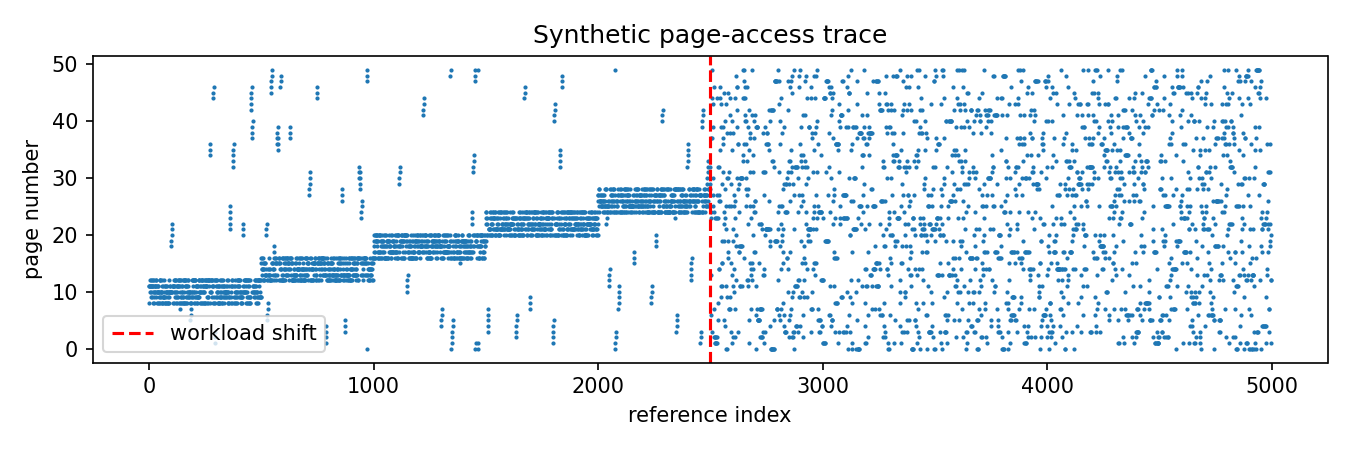
\includegraphics[width=\linewidth]{../results/fig_trace.png}
\caption{Synthetic reference trace showing the deliberate workload shift.}
\label{fig:trace}
\end{figure}

\section{Results}
The most useful comparison is the 8-frame case because it gives enough memory to exploit locality while still forcing substantial replacement. The classical policies achieved the following hit ratios:

\begin{center}
\begin{tabular}{lrrr}
\toprule
Policy & Before & After & Drop\\
\midrule
FIFO & 0.834 & 0.349 & 0.486\\
LRU & 0.867 & 0.350 & 0.517\\
Learned (static) & 0.896 & 0.344 & 0.552\\
Learned (both phases) & 0.714 & 0.318 & 0.396\\
Optimal & 0.914 & 0.561 & 0.353\\
\bottomrule
\end{tabular}
\end{center}

For completeness, changing the number of frames changes the absolute performance substantially. With 4 frames, LRU falls from 0.672 to 0.298, while Optimal falls from 0.808 to 0.428. With 16 frames, LRU falls from 0.914 to 0.477 and Optimal from 0.945 to 0.721. Thus, more physical frames reduce the damage from the workload shift, although the phase change is still visible.

\begin{figure}[ht]
\centering
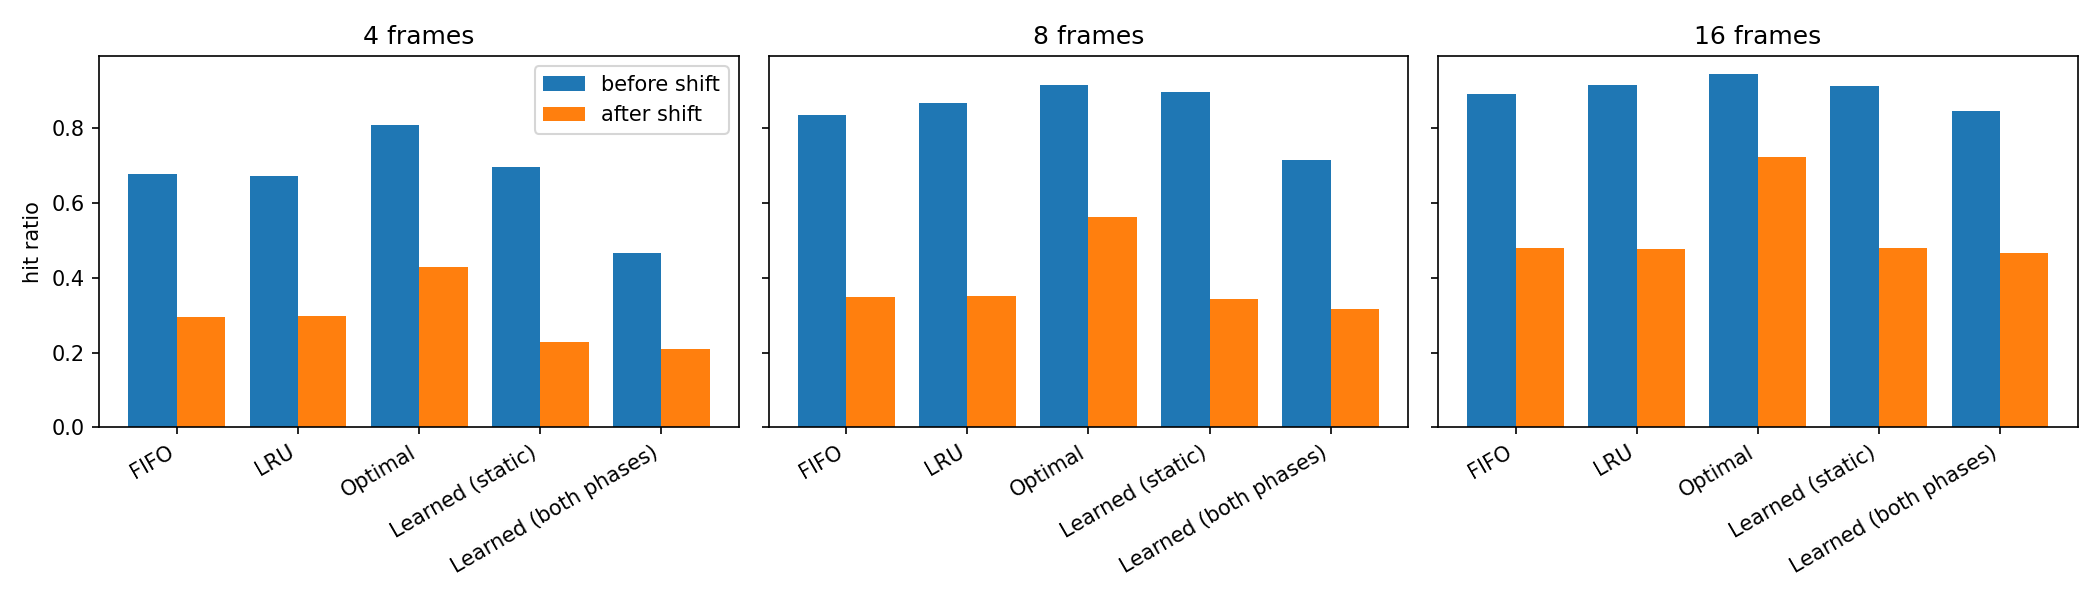
\includegraphics[width=\linewidth]{../results/fig_hit_ratio_before_after.png}
\caption{Hit ratio before and after the workload shift.}
\label{fig:hit}
\end{figure}

\begin{figure}[ht]
\centering
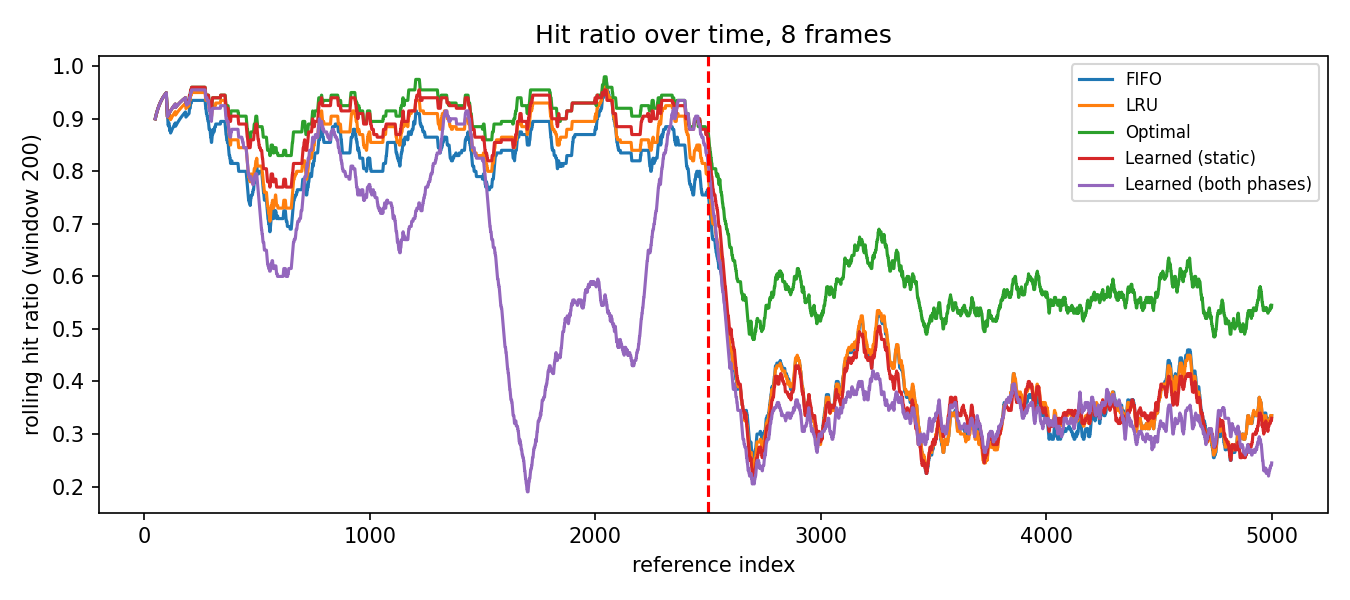
\includegraphics[width=\linewidth]{../results/fig_rolling_hit_ratio.png}
\caption{Rolling hit ratio across the trace.}
\label{fig:rolling}
\end{figure}

\section{Analysis: What Changed Under the Shift and Why}
The largest classical-policy degradation at 8 frames is LRU: its hit ratio falls by 0.517. This is expected because phase 1 was deliberately designed to make recency informative. The working set is small and moves slowly, so pages referenced recently tend to remain useful. After the shift, the workload becomes much less predictable. Under mostly random access, being recently referenced does not imply that the same page will be referenced again soon. A page can be used once and then disappear from the workload for a long time, while an older page can become the next useful page by chance.

The static learned model shows the same problem more strongly. At 8 frames it has the best pre-shift hit ratio of 0.896 among the non-Optimal policies, but drops to 0.344 after the shift. Its 0.552 drop is the largest in the table. This demonstrates a limitation of learning from a single workload regime: the model learns relationships that are useful when locality is stable, but those relationships do not necessarily transfer when the access distribution changes.

The both-phases model is more conservative across the shift. Its pre-shift hit ratio is lower (0.714), but its drop is smaller (0.396). This does not mean that it has learned a superior replacement strategy. Instead, training on both behaviours prevents the model from being specialized only to the highly local phase. In this experiment it still performs below LRU after the shift, showing that the three simple features are not sufficient to recover the information that is lost when future reuse becomes unpredictable.

The post-shift results also show why random access places a natural limit on all replacement policies. With 50 pages, a purely uniform random reference would give a simple baseline near frames/50 for the probability that the next reference is already resident: about 0.08, 0.16 and 0.32 for 4, 8 and 16 frames. The measured values are higher because the second phase is not perfectly uniform; it includes occasional bursts on three hot pages, which create short-lived locality that replacement policies can exploit. Nevertheless, the policies become much closer to one another than they were in phase 1. Once the past contains little reliable information about the future, sophisticated recency decisions have less advantage.

Optimal remains clearly better after the shift, especially with 16 frames (0.721 versus about 0.48 for FIFO/LRU/learned). This gap is expected: Optimal is explicitly given the future and can preserve pages that will be needed soon. Its smaller degradation, particularly the 0.224 drop at 16 frames, also shows that some of the post-shift difficulty comes from the uncertainty faced by online policies rather than simply from insufficient memory.

Overall, the experiment supports a practical conclusion: replacement heuristics work best when workload behaviour has enough temporal structure for past observations to predict future reuse. A workload shift can invalidate those patterns. Retraining on a broader mixture can reduce specialization, but simple features alone do not guarantee robustness.

\section{Bonus: Explanation Confidence}
The bonus evaluation does not support a claim that the model is well calibrated. Across all 1,894 logged eviction decisions, accuracy is 0.188, while mean confidence is about 0.484 for correct decisions and 0.479 for incorrect decisions. After the shift, accuracy falls to 0.160 while mean confidence remains about 0.485 for correct decisions and 0.483 for wrong decisions.

The calibration table makes the problem clearer. In the 0.4--0.6 confidence bin, the model reports a mean confidence of 0.565 but achieves only 0.193 actual accuracy. Therefore, confidence is much higher than the observed probability of being correct. The model is consequently overconfident and poorly calibrated. The result is useful because it shows that producing a probability-like score is not the same as producing a trustworthy probability estimate.

\begin{figure}[ht]
\centering
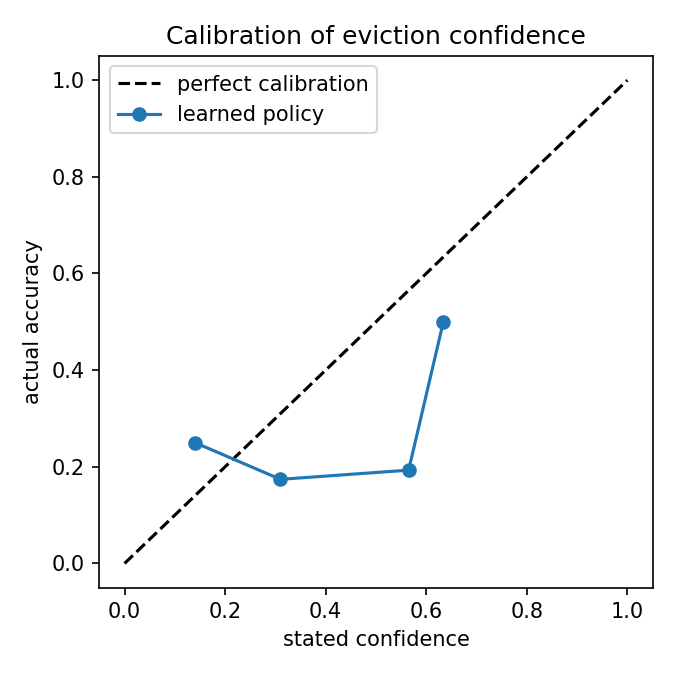
\includegraphics[width=\linewidth]{../results/fig_calibration.png}
\caption{Confidence calibration for the learned eviction decisions.}
\label{fig:cal}
\end{figure}

\section{Conclusion}
The experiment demonstrates the effect of workload shifts on page replacement. FIFO and LRU exploit phase-1 locality effectively, but their hit ratios drop sharply when the trace becomes mostly random and bursty. LRU's strong pre-shift performance does not protect it from this change because recency becomes a weak predictor of future reuse. The learned policy can reproduce useful locality-related behaviour when trained on a matching workload, but its performance also degrades when the workload distribution changes. Training on both phases reduces the size of the shift-related drop, although it sacrifices phase-1 performance and still does not outperform LRU after the shift.

The bonus experiment reinforces the same lesson from a machine-learning perspective: confidence from a classifier should not automatically be treated as reliable evidence. In this implementation, confidence is poorly calibrated and remains high even when decision accuracy is low. Overall, the results show that page replacement quality depends strongly on workload characteristics and that robustness under changing workloads is a separate challenge from achieving high accuracy on a stable workload.

\begin{thebibliography}{9}
\bibitem{belady} L.~A.~Belady, ``A study of replacement algorithms for a virtual-storage computer,'' \emph{IBM Systems Journal}, vol.~5, no.~2, pp.~78--101, 1966.
\bibitem{silberschatz} A.~Silberschatz, P.~B.~Galvin, and G.~Gagne, \emph{Operating System Concepts}, 10th ed., Wiley, 2018.
\bibitem{sklearn} F.~Pedregosa et al., ``Scikit-learn: Machine learning in Python,'' \emph{Journal of Machine Learning Research}, vol.~12, pp.~2825--2830, 2011.
\end{thebibliography}
\end{document}
